\usepackage[magyar]{babel}
\usepackage[T1]{fontenc}
\usepackage[utf8]{inputenc}
\usepackage{graphicx}
\usepackage{listings}
\usepackage{amsmath}
\usepackage{amssymb}
%\usepackage{amsthm}
\usepackage{ae,aecompl}

\usetheme{Goettingen}
%\usetheme{Singapore}

%\theoremstyle{plain}
\newtheorem{thm}{Tétel}[section]
\newtheorem{thmsub}{Tétel}[subsection]
\newtheorem{lem}[thm]{Lemma}
\newtheorem{lemsub}[thmsub]{Lemma}
\newtheorem{all}[thm]{Állítás}
\newtheorem{allsub}[thmsub]{Állítás}
\newtheorem{kov}[thm]{Következmény}
\newtheorem{sej}[thm]{Sejtés}

%\theoremstyle{definition}
\newtheorem{defn}[thm]{Definíció}
\newtheorem{defnsub}[thmsub]{Definíció}
\newtheorem{jel}[thm]{Jelölés}

%\theoremstyle{remark}
\newtheorem{alg}[thm]{Algoritmus}
\newtheorem{megj}[thm]{Megjegyzés}
\newenvironment{biz}{Bizonyítás: }{$\square$}
\newcommand{\leftexp}[2]{{\vphantom{#2}}^{#1}{#2}}

\title{3 dimenziós D-szimbólumok és a Thurston-sejtés}
\author{Boróczki Lajos}
\date{2011. október 25.}

\begin{document}

\begin{frame}
  \maketitle
\end{frame}

\begin{frame}
  \mode<presentation>{\frametitle{Kivonat}}
  \tableofcontents
\end{frame}
\newpage

\section{D-szimbólum felépítése}
\begin{frame}
  \frametitle{D-szimbólum, mint új nyelvezet}
  \begin{itemize}
    \item Kompakt alaptartományú kövezés baricentrikus felbontása
    \item Szomszédsági operációk \mode<article>{Következő lépésként bevezetünk
      szomszédsági operációkat az előbb előállított baricentrikus szimplexekre:
      $\sigma_0,\sigma_1,\ldots,\sigma_d.$ Az operációk jelentése: $\sigma_i(C)$
      a $C\in \mathcal{C}$ szimplex azon szomszédja, amely az $i$-lapja, azaz az
      $i$. csúccsal szemközti lap mentén szomszédos $C$-vel.  Minden $\sigma_i$
      operáció egy involúció a fent leírt szimplexek $\mathcal{C}$ halmazán.}
      Jelölés:\\<all>
\setlength{\unitlength}{1cm}
$\sigma_0$:
\begin{picture}(1,0.2)
  \multiput(0,0.1)(0.2,0){5}{\circle*{0.001}}
\end{picture},
$\sigma_1$:
\begin{picture}(1,0.2)                                                                                 
  \multiput(0,0.1)(0.25,0){4}{\line(1,0){0.15}}                                                        
\end{picture},
$\sigma_2$:
\begin{picture}(1,0.2)
  \put(0,0.1){\line(1,0){1}}
\end{picture},
$\sigma_3$:
\begin{picture}(1.5,0.2)
  \multiput(0,0.1)(0.5,0){3}{\line(1,0){0.2}}
  \multiput(0.35,0.1)(0.5,0){3}{\circle*{0.001}}
\end{picture}
    \item Egybevágóság csoport szerinti szimplex pályák halmaza
      \mode<article>{Általában megkövetelhetjük, hogy a kövezésnek egy
      egybevágóság csoportja változatlanul hagyja a kövezés kombinatorikus
      struktúráját, így a baricentrikus felbontást is. Vehetjük az egybevágóság
      csoport szerinti szimplex pályák halmazát, ezeken is jól értelmezett lesz
      a szomszédsági operáció.}
    \item $(d-2)$-lap körüli szimplex pályák. \mode<article>{Következő lépésként
      vizsgáljuk meg, hogy egy $(d-2)$-lap körül ($3$ dimenzióban él körül) hány
      baricentrikus szimplex ($\mathcal{M}$ mátrix-függvény értékeinek duplája)
      illetve hány szimplex pálya ($\mathcal{R}$ mátrix-függvény értékek
      duplája) csatlakozik.}
    \item Egyértelműség: A baricentrikus felbontásban csak az alaptartomány
      csúcspontjaihoz tartozó szimplex csúcsok lehetnek végtelen távoli pontok,
      ezért minden kövezés leírható D-szimbólummal és ez permutáció erejéig
      egyértelmű. FIXME: Miért nem foglalkozunk azzal az esettel, amikor egy
      egész él végtelen távol van?
  \end{itemize}
\end{frame}

\subsection{Példa}
\begin{frame}
  Az $\mathbb{E}^3$ tér négyzetes hasábbal történő egyik legegyszerűbb
  térkitöltése. Baricentrikus felbontása és a szimplex pályákhoz tartozó
  multigráf: \mode<article>{\ref{abra:hasab_bari}.
  ábra. Mivel minden szimplex pályára definiálva van minden szomszédsági
  reláció, ezért az áttekinthetőség kedvéért azokat a hurok relációkat nem ábrázoljuk,
  melyek sík tükrözéssel önmagára képezik le a pályát.}
  \begin{figure}
    \mode<article>{\caption{\label{abra:hasab_bari} Piros:1, kék:2, zöld:3}}
    \center
    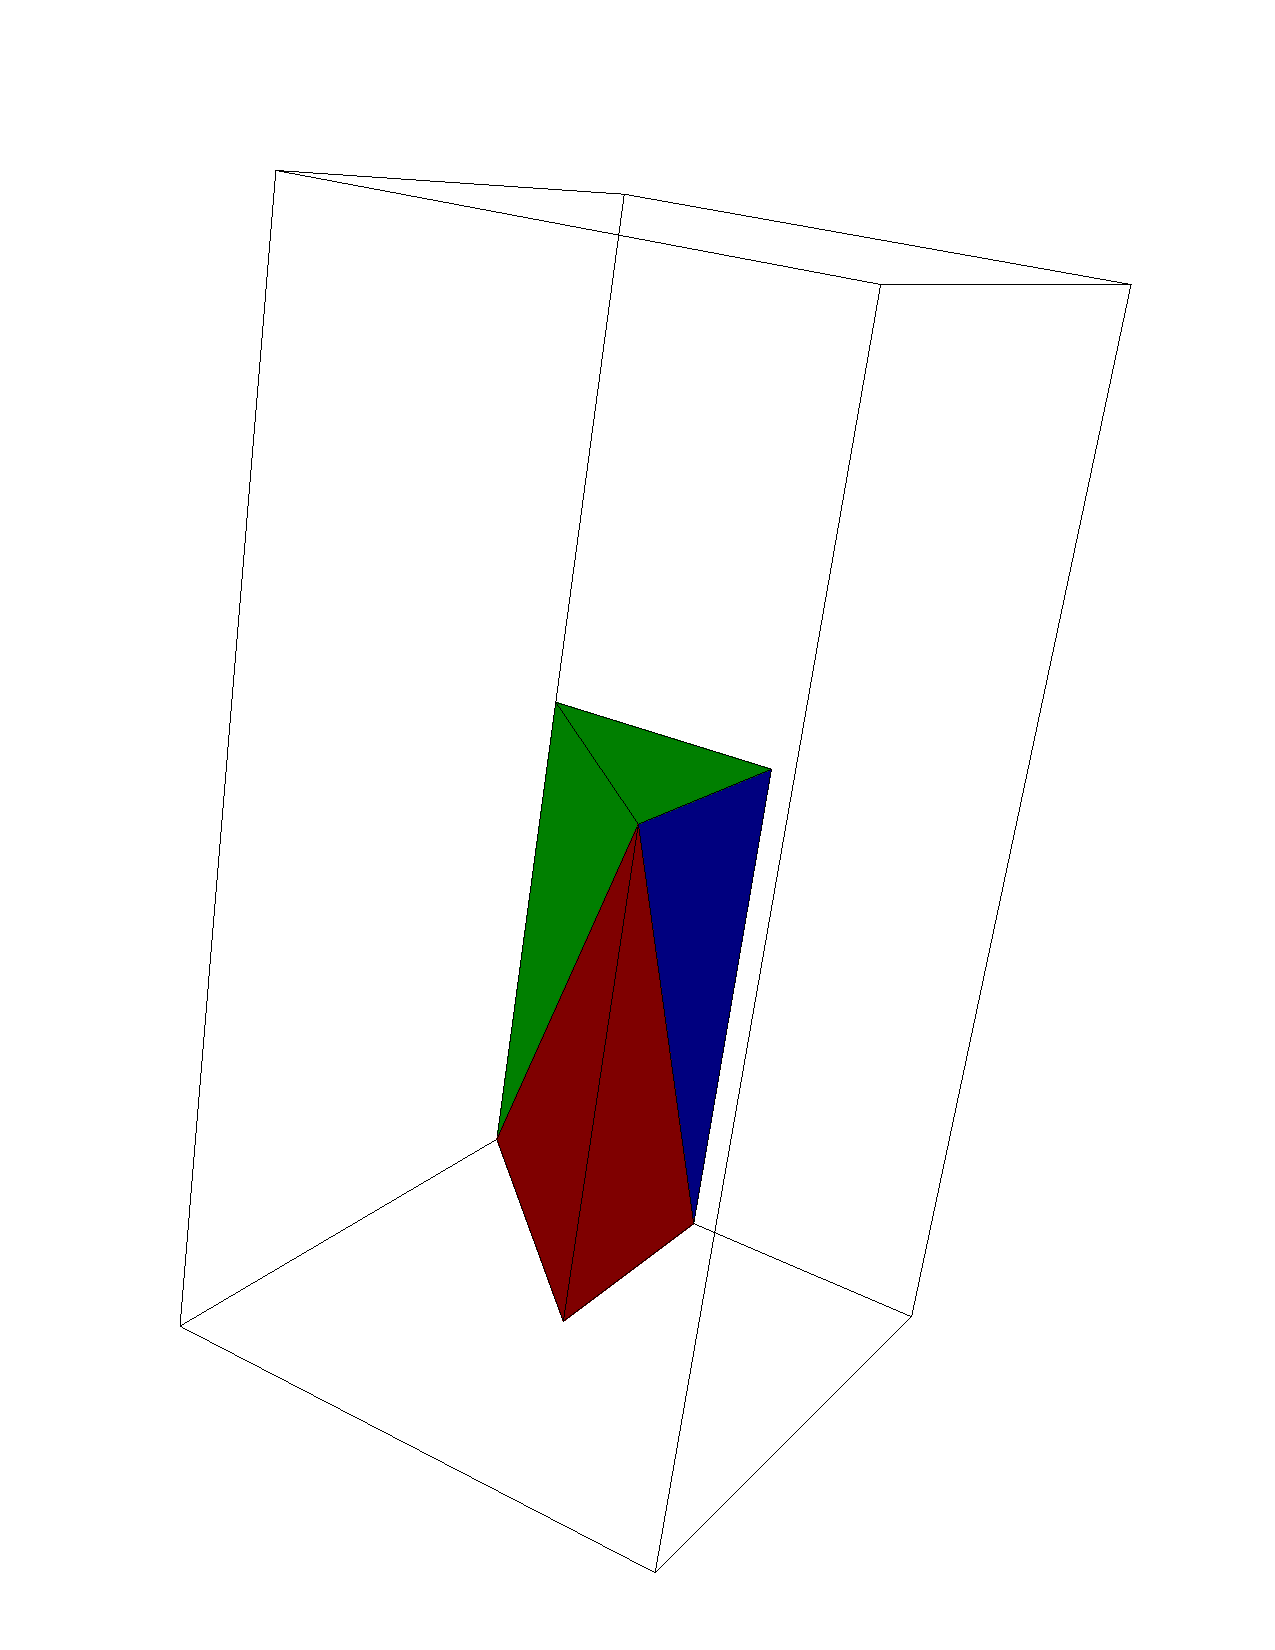
\includegraphics[width=0.4\textwidth]{hasab_bari.pdf}
    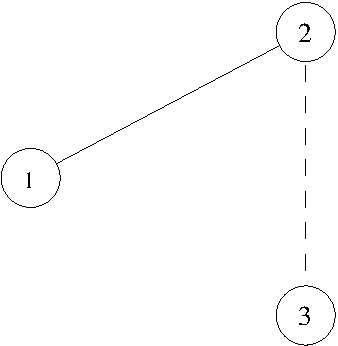
\includegraphics[width=0.35\textwidth]{hasab_D-graf.pdf}
  \end{figure}
\end{frame}

\begin{frame}
  A mátrixfüggvények ($\mathcal{D}$ a szimplex pályák halmaza,
  $D_i\in\mathcal{D}$):
  \begin{equation*}
    \mathcal{R}(D_1)=
    \left(
    \begin{array}{cccc}
      1 & 1 & 2 & 1\\
      1 & 1 & 3 & 1\\
      2 & 3 & 1 & 2\\
      1 & 1 & 2 & 1
    \end{array}
    \right)
  \end{equation*}
  \begin{equation*}
    \mathcal{R}(D_2)=
    \left(
    \begin{array}{cccc}
      1 & 2 & 2 & 1\\
      2 & 1 & 3 & 2\\
      2 & 3 & 1 & 2\\
      1 & 2 & 2 & 1
    \end{array}
    \right)
  \end{equation*}
  \begin{equation*}
    \mathcal{R}(D_3)=
    \left(
    \begin{array}{cccc}
      1 & 2 & 1 & 1\\
      2 & 1 & 3 & 2\\
      1 & 3 & 1 & 1\\
      1 & 2 & 1 & 1
    \end{array}
    \right)
  \end{equation*}

  \begin{equation*}
    \forall D_i\in\mathcal{D}:\;
    \mathcal{M}(D_i)=
    \left(
    \begin{array}{cccc}
      1 & 4 & 2 & 2\\
      4 & 1 & 3 & 2\\
      2 & 3 & 1 & 4\\
      2 & 2 & 4 & 1
    \end{array}
    \right)
  \end{equation*}
\end{frame}

\section{Lehetséges D-szimbólumok}
\subsection{Feltételek}
\begin{frame}
  D-szimbólum: $(\Sigma_I,\mathcal{D},\mathcal{M})$ hármasok. \mode<article>{Az
  alábbi feltételeknek megfelelő $(\Sigma_I,\mathcal{D},\mathcal{M})$ hármasokat
  nevezzük Delone-Delaney-Dress szimbólumnak, röviden D-szimbólumnak.}
  \begin{itemize}
    \item Természetes feltételek D-diagramokra\mode<article>{ (mivel kövezések baricentrikus
      felbontásainak leírására használjuk őket.)}:
      \begin{enumerate}
	\item $\mathcal{D}$ véges
	\item A szimplex pályákon értelmezett szomszédsági operációk involutív
	  permutációk\mode<article>{, vagyis $\forall i\in I, \sigma_i\in
	  \Sigma_I, \forall D\in \mathcal{D}$:
	  \begin{align*}
	    \sigma_i\sigma_i(D)=D 
	  \end{align*}
	  A diagram minden csúcsában az azonos
	  színű élek foka 1 vagy 2. A fok pontosan akkor 2, ha az él egy hurok
	  (kezdő és végpontja azonos.)}
	\item Nem szomszédos operáció-párokat alkalmazva legfeljebb $2$ lépésből
	  visszajutunk a kiindulási csúcsba\mode<article>{. \newline $\forall
	  i,j\in I, \forall D\in \mathcal{D}$:
	  \begin{align*}
	    |i-j|\geq 2 \Rightarrow (\sigma_j\sigma_i)^2(D)=D
	  \end{align*}}
      \end{enumerate}
    \item Bevezetjük a szimplex pályákon (D-diagram csúcsokon) értelmezett $\mathcal{R}$
      mátrix-függvényt\mode<article>{.
	\newline $\forall i,j\in I, \forall D\in \mathcal{D}$:
      \begin{align*}
	r_{ij}(D)=r_{ji}(D)=\mathrm{min}\left\{r\in \mathbb{N}^+|(\sigma_j\sigma_i)^r(D)=D\right\}
      \end{align*}
      A D-diagram feltételei $\mathcal{R}$ mátrix-függvényre vetítve:
      $r_{ii}(D)=1$, illetve $|i-j|\geq 2 \Rightarrow r_{ij}(D)\leq2$}
    \item Feltételek a diagramhoz tartozó $\mathcal{M}$ mátrix-függvényre:
      \begin{enumerate}
	\item Az $\mathcal{R}$ mátrix-függvény minden elemének osztania kell az
	  $\mathcal{M}$ mátrix-függvény megfelelő elemét.
	  \mode<article>{
	  Csak így biztosítható, hogy egy $d-2$ dimenziós lap ($3$ dimenzióban él)
	  teljes körüljárásakor azonos szimplex pályába érkezünk; ami pedig szükséges
	  ahhoz, hogy azonos szimplexbe érkezhessünk. Az $\mathcal{M}$ és
	  $\mathcal{R}$ mátrix-függvények értékeinek hányadosa a kövezés
	  periodicitását mutatja az adott él körül.
	  \newline $\forall i,j\in I, \forall D\in \mathcal{D}$:
	  $r_{ij}(D)|m_{ij}(D)$
	  }
	\item Pálya feltétel\mode<article>{. Minden operáció-párhoz és
	  kiindulási diagram-csúcshoz definiálhatjuk a hozzá tartozó pályát: az
	  összes diagram-csúcs, amit érintünk miközben az operációkat
	  elvégezzük. Az $\mathcal{M}$ mátrix-függvény értékeinek egy-egy pályán belül
	  meg kell egyeznie, különben a kapott kövezésben függne az él körüli
	  szimplexek száma a kezdő szimplextől. A pályát visszafelé bejárva is
	  ugyanazt az utat kell megtennünk, ezért az $\mathcal{M}$
	  mátrix-függvény mátrixai szimmetrikusak.
	  \begin{align*}
	    &\forall i,j\in I, \forall D\in \mathcal{D} \\
	    &\mathcal{D}'=\left\{(\sigma_j\sigma_i)^k(D)|k\in
	    \mathbb{N}\right\}\cup\left\{\sigma_i(\sigma_j\sigma_i)^k(D)|k\in
	    \mathbb{N}\right\}\\
	    &\forall D_1,D_2 \in \mathcal{D}'\\
            &m_{ij}(D_1)=m_{ij}(D_2)=m_{ji}(D_1)=m_{ji}(D_2)
	  \end{align*}
	  }
	\item Az $\mathcal{M}$ mátrix-függvény minden mátrixának főátlójától legalább
	  2 távolságra lévő helyeken $2$-esek állnak\mode<article>{, különben nem
	  kapjuk vissza a baricentrikus felbontást.
	  \newline $\forall i,j\in I, \forall D\in \mathcal{D}$:
	  \begin{align*}
	    m_{ij}(D)=2
	  \end{align*}}
	\item A főátlótól $1$ távolságra lévő helyeken a mátrix-függvény értékei
	  legyenek nagyobbak vagy egyenlőek, mint 2\mode<article>{. Egyenlőség esetén
	  degenerált, illetve mesterkélt esetekhez jutunk, melyekben például
	  digonok is lehetnek lapok. (Szép kövezés esetén egy 3 dimenziós poliéder bármely
	  csúcsában legalább 3 él és 3 lap találkozik, minden lapnak legalább 3
	  oldaléle van, minden élnél legalább 3 test és 3 lap fut össze.)
	  \newline $\forall i\in I-\{0\}, \forall D\in \mathcal{D}$:
	  \begin{align*}
	    m_{i(i-1)}(D)\geq 2
	  \end{align*}}
      \end{enumerate}
  \end{itemize}
\end{frame}

Az eddigi megállapítások szükséges (de nem mindig elégséges)
feltételek olyan $d$ dimenziós (nem feltétlenül euklideszi) térkitöltés
létezésére (amelynek D-szimbóluma $(\Sigma_I,\mathcal{D},\mathcal{M})$.) Most nézzük
speciálisan a 3 dimenziós eset további követelményeit.

\subsection{Rész D-szimbólum}
\begin{frame}
  Rész D-szimbólum:
  \begin{itemize}
    \item Az i-edik komponens vagy rész D-szimbólum
      $(\Sigma_I^i,\mathcal{D}^i,\mathcal{M}^i)$ jelentése\mode<article>{: az i-edik
      operációt elhagyjuk a diagramból illetve a mátrix-függvény soraiból és
      oszlopaiból is.}
    \item A kombinatorikus görbületi függvény számolható\mode<article>{. A rész
      D-szimbólum komponenseihez tartozó kövezésben a D-szimbólum alapján
      felírható a kombinatorikus görbületi függvény:}
      \begin{align*}
	K(\leftexp{c}{\mathcal{D}}^i)=\sum_{D\in
	\leftexp{c}{\mathcal{D}}^i}\left(-1+\sum_{\substack{0\le j<k\le d \\
	j,k\ne i}}\frac{1}{m_{jk}(D)}\right)
	\begin{array}{cccc}
	  > & & S^2 \\
	  = & 0 & \mathbb{E}^2 \\
	  < & & H^2
	\end{array}
      \end{align*}
      \mode<article>{Ez alapján eldönthető, hogy a 3 lehetséges felület közül melyiken valósul
      meg.}
    \item Vizuális jelentés\mode<article>{: A rész D-szimbólum vizuális
      jelentése az adott i-indexű csúcs körüli 1-gyel kisebb dimenziós felületen
      létrehozott $(3-1)$-dimenziós kövezés D-szimbóluma az i-indexű csúcs
      stabilizátora szerint.  Ezért egy i-indexű valódi szimplex-csúcs körüli
      rész D-szimbólum egy szférikus kövezéshez kell tartozzon, egy ideális
      szimplex-csúcs körül euklideszi kövezés alakul ki pl. a hiperbolikus tér
      paraszféra (horoszféra) felületén; a hiperbolikus síkkövezéseket
      kizárjuk, mert modellen kívüli (végtelennél távolabbi) pontot, mint
      i-csúcsot jellemezne.}
    \item Jó orbifold feltétel\mode<article>{: Szférikus síkon történő
      kövezésnek további feltétele, hogy az úgy nevezett  rossz orbifoldokat
      kizárjuk, azaz a következő lehetőségek hibásak (Convay illetve
      Macbeath-féle jelöléseik alapján):
      \begin{align*}
	u=(+,0;[u];\{\}), & & 1<u;\\
	*u=(+,0;[];\{(u)\}), & & 1<u;\\
	uv=(+,0;[u,v];\{\}), & & 1<u<v;\\
	*uv=(+,0;[];\{(u,v)\}), & & 1<u<v.
      \end{align*}
      Ezek a csepp felületekre illetve az észak-déli póluson nem azonosan viselkedő
      gömb felületekre utalnak.}
  \end{itemize}
\end{frame}

\begin{frame}
  További követelmények a rész D-szimbólumok alapján:
  \begin{enumerate}
    \item $(\Sigma_I^1,\mathcal{D}^1,\mathcal{M}^1)$ és
      $(\Sigma_I^2,\mathcal{D}^2,\mathcal{M}^2)$ esetén a
      görbületi függvény pozitív és a jó orbifold feltétel
      teljesül\mode<article>{. Élközépponthoz és lapközépponthoz tartozó
      szimplex csúcs valódi csúcs kell legyen, ezért egy $S^2$-n megvalósuló
      kövezést kell kapjunk.}
    \item $(\Sigma_I^0,\mathcal{D}^0,\mathcal{M}^0)$ és
      $(\Sigma_I^3,\mathcal{D}^3,\mathcal{M}^3)$ esetén a görbületi függvény
      pozitív és a jó orbifold feltétel teljesül, vagy a görbületi függvény
      $0$\mode<article>{. Csúcshoz és test-középponthoz tartozó szimplex csúcs
      lehet valódi, ekkor egy $S^2$-n megvalósuló kövezést kell kapjunk; vagy
      lehet ideális, ekkor $\mathbb{E}^2$-n megvalósuló kövezést kell kapjunk.
      (Az ideális test-középpont esetét a dualitás miatt meghagyjuk; de
      megjegyezzük, hogy a végtelen poliéderekkel történő kövezés nem igazán
      érdekes (egy kisebb dimenziós felület kövezésének felel meg.))}
  \end{enumerate}
\end{frame}


\section{D-szimbólumok felsorolása}
\begin{frame}
  D-szimbólumok felsorolása:
  \begin{itemize}
    \item Nagyravágyó terv\mode<article>{: Az összes $n$-dimenziós geometriában
      az összes lehetséges véges alaptartományú kövezés felsorolásához
      szeretnénk a D-szimbólumokat felhasználni.}
    \item Alapvetően nem tűnik lehetetlennek\mode<article>{, mivel a
      D-szimbólumokat minden olyan kövezésre értelmezhetjük, ahol tudunk
      baricentrikus felbontást végezni.}
    \item Nagyon sok lehetőség van\mode<article>{: a dimenzió és a D-diagram
      elemszámának méretében is exponenciális}
    \item Rendezés a D-diagramokon, algoritmus a felsorolásukra
    \item Rendezés a mátrix-függvényeken, $3$-dimenziós esetben algoritmus a
      lehetséges mátrix-függvények felsorolására \mode<article>{ az előző
      fejezetben felsorolt feltételeknek megfelelően. A két kulcs a paraméteres
      megadás és a rész D-szimbólum által indukált felső korlát (de a végtelen
      láncokat kezelni kell.)}
    \item A 12 elemszámú D-szimbólumokat tudjuk jelenleg felsorolni.
  \end{itemize}
\end{frame}

\section{Éltranzitív kövezések}
\begin{frame}
  Éltranzitív kövezések kezelése D-szimbólummal
  \begin{itemize}
    \item Egyszerű új feltétel: a diagramban nem lehet 1-es színű (szaggatott)
      él
    \item A lehetséges diagramok végigpróbálgatása egyszerűbbé válik
    \item 18-as elemszámig jutottunk, és ismert, hogy legfeljebb 24 elemszámú
      ilyen diagramok lehetségesek.
  \end{itemize}
\end{frame}

\section{Splitting probléma és a Thurston-sejtés (támadása)}
\begin{frame}
  Thurston sejtés:
  \begin{itemize}
    \item Minden irányított, primitív, zárt 3-sokaság felvágható (splitting)
      tórusz ($E^2$) felületek mentén úgy, hogy a kapott sokaságok belsejének
      geometriai struktúrája van, melynek véges a térfogata.
    \item A következő 8 féle maximális modell-geometria létezik, amihez van
      kompakt sokaság, ami az adott geometriában modellezhető: $S^3$, $E^3$,
      $H^3$, $S^2\times R$, $H^2\times R$, $\widetilde{SL2R}$, Sol,
      Nil.
  \end{itemize}
  Megjegyzések:
  \begin{itemize}
    \item A nem irányítható eset kezelhető az ,,irányítható dupla fedés''
      módszerrel, ami az M sokasághoz rendelt $M\times Z/2Z$ sokaság
      (értelmes visszahúzó operációval). \mode<article>{Például Möbius szalaghoz
      rendelhetünk egy dupla Möbius szalagot úgy, hogy felvágjuk valahol és
      betoldunk mégegy Möbius szalagot. Ezzel egy gyűrű alakot kapunk.}
    \item A 2 dimenziós analógia: minden határ nélküli felületnek (2-sokaságnak)
      geometriai struktúrája van, konstans görbületű metrikával.
  \end{itemize}
\end{frame}

\begin{frame}
  Splitting keresése D-szimbólumban
  \begin{itemize}
    \item $S^2$ jellegű splitting: Ponttá zsugorítható részlet a kövezésben,
      ezáltal \mode<article>{kevesebb szimplex-csúcsból, így} kevesebb
      szimplex-pályából álló kövezéssel ekvivalenset kapunk. (Rossz orbifold
      probléma itt is felléphet.)
      FIXME Rajz
    \item $E^2$ splitting: A Thurston sejtés-beli splittingnek megfelelő dolog.
      Végtelen távoli pontba tolható.
      FIXME Rajz
  \end{itemize}
\end{frame}

\begin{frame}
  További feltételek a Thurston sejtés-beli minimális 3-sokaságokra
  \begin{itemize}
    \item Az ábrákon látszik, hogy a megfelelő 2 sokaságokra a kombinatorikus
      görbület függvényt felírva alsó korlátot is kapunk a paramétereinkre.
      FIXME Fontos kérdés, hogy ez elég-e.
    \item A D-diagram alapján felírhatóak a szimplex csúcsok (rész D-diagram) és
      a szimplex csúcsok közti élek is. Ezeket gráfnak tekintve az összes
      lehetséges 2 (legalább 2 elemű) partícióra bontást meg kell vizsgálni.
    \item Az így kapott "splitting-jelölt" helyet meg kell vizsgálni, hogy
      megkapjuk az összes alsó korlátot a paraméterekre.
    \item A kapott D-szimbólumok minimálisak abban az értelemben, hogy nincs
      bennük se $E^2$ se $S^2$ splitting. (Ha találunk köztük olyat, ami nem
      realizálható a 8-féle geometriában, akkor a Thurston-sejtést sikeresen
      támadtuk.)
  \end{itemize}
\end{frame}

\end{document}
